\subsection{K-nearest neighbours}

The data set has been exposed to classification by looking at the k nearest neighbours.

\begin{figure}
	\begin{subfigure}[b]{0.5\textwidth}
	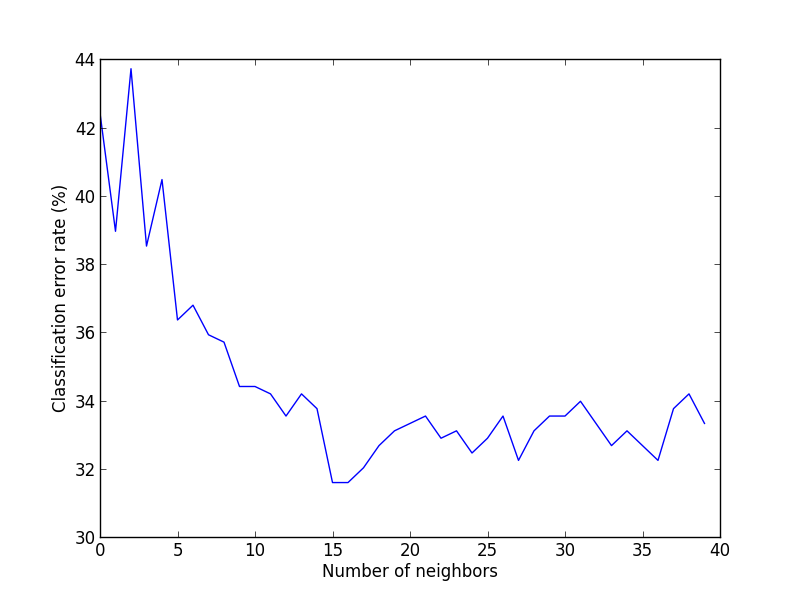
\includegraphics[scale=0.4]{pictures/knnX.png}
	\caption{Looking at all attributes.}
	\label{logicalRegressionResultX}
	\end{subfigure}
	\begin{subfigure}[b]{0.5\textwidth}
	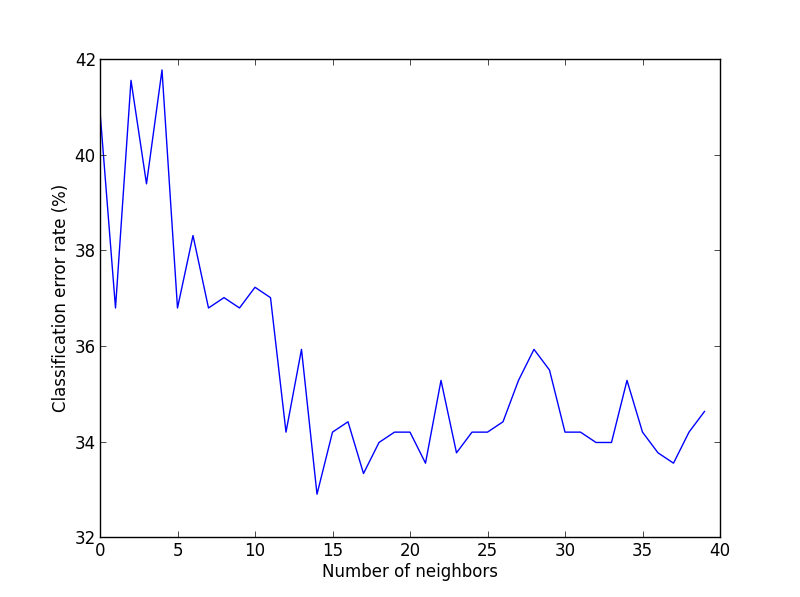
\includegraphics[scale=0.4]{pictures/knnXAD.png}	
	\caption{Looking at attributes selected by forward selection.}
	\label{logicalRegressionResultXad}
	\end{subfigure}

	\begin{subfigure}[b]{0.5\textwidth}
	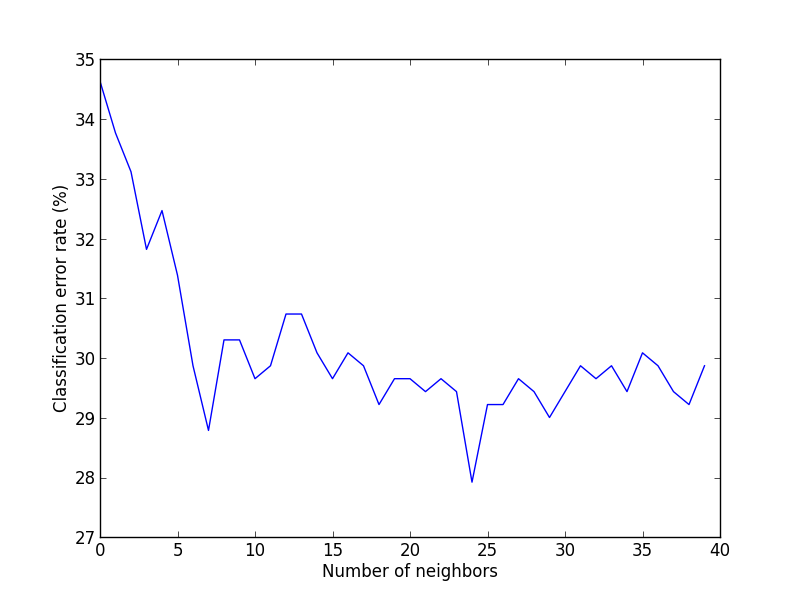
\includegraphics[scale=0.4]{pictures/knnPC.png}
	\caption{Looking at all principal components.}
	\label{logicalRegressionResultXPA}
	\end{subfigure}
	\begin{subfigure}[b]{0.5\textwidth}
	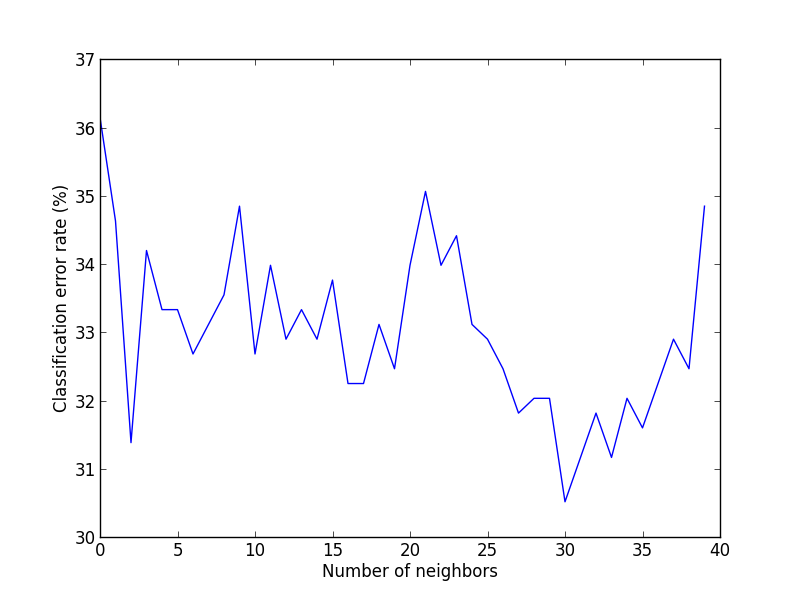
\includegraphics[scale=0.4]{pictures/knn2PC.png}
	\caption{Looking at two most important principal components.}
	\label{logicalRegressionResultX2PA}
	\end{subfigure}
\caption{This figure shows results of performing logical regression for different input.}
\label{logicalRegressionResults}
\end{figure}


\begin{figure}
	\begin{subfigure}[b]{0.5\textwidth}
	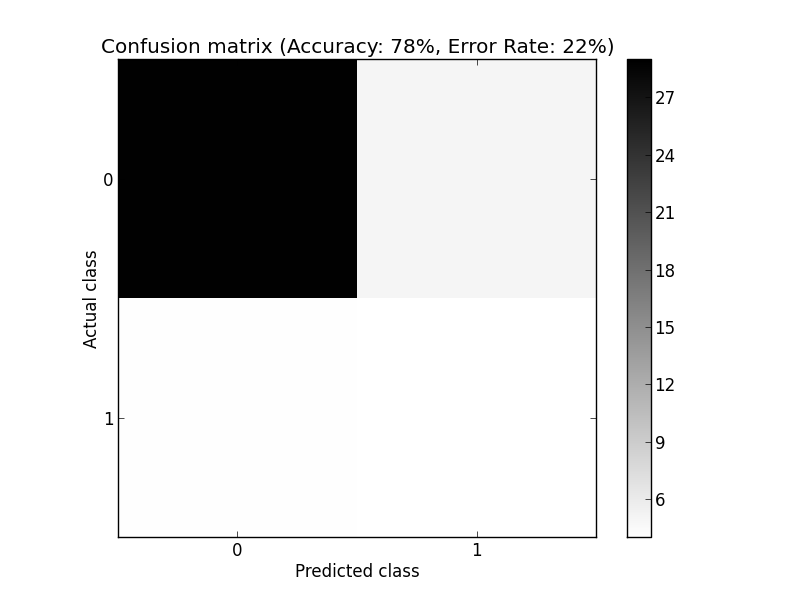
\includegraphics[scale=0.4]{pictures/cmX.png}
	\caption{Looking at all attributes.}
	\label{logicalRegressionResultX}
	\end{subfigure}
	\begin{subfigure}[b]{0.5\textwidth}
	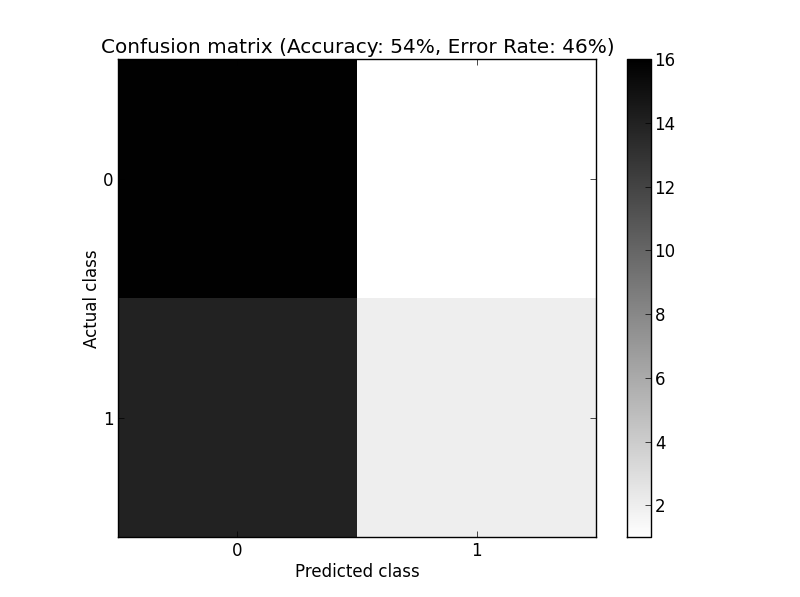
\includegraphics[scale=0.4]{pictures/cmXAD.png}	
	\caption{Looking at attributes selected by forward selection.}
	\label{logicalRegressionResultXad}
	\end{subfigure}

	\begin{subfigure}[b]{0.5\textwidth}
	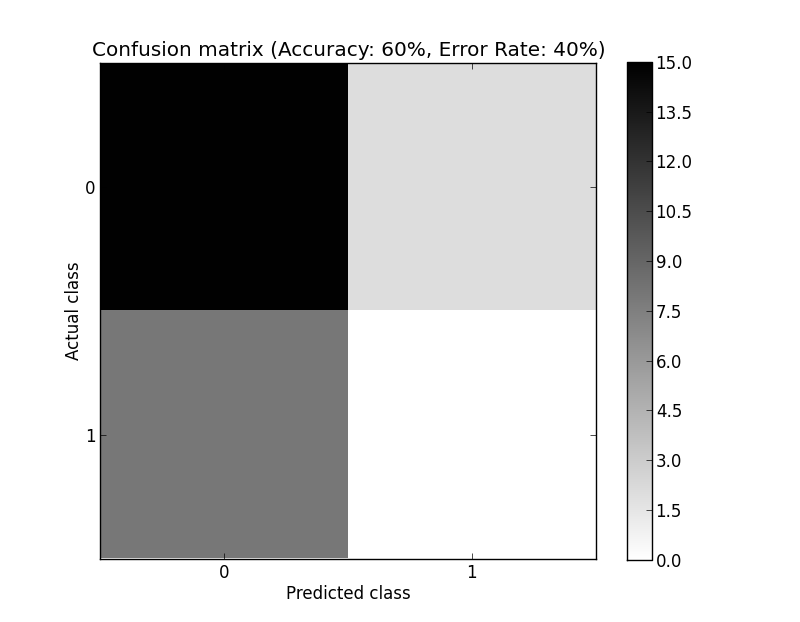
\includegraphics[scale=0.4]{pictures/cmPC.png}
	\caption{Looking at all principal components.}
	\label{logicalRegressionResultXPA}
	\end{subfigure}
	\begin{subfigure}[b]{0.5\textwidth}
	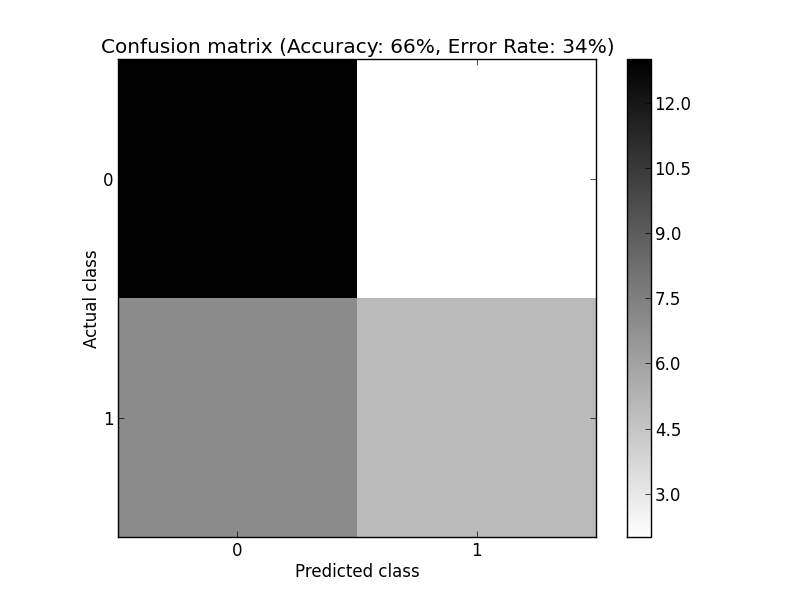
\includegraphics[scale=0.4]{pictures/cm2PC.png}
	\caption{Looking at two most important principal components.}
	\label{logicalRegressionResultX2PA}
	\end{subfigure}
\caption{This figure shows results of performing logical regression for different input.}
\label{logicalRegressionResults}
\end{figure}

